\documentclass[a4paper,11pt,UTF8]{article}
\usepackage{ctex}
\usepackage{amsmath,amsthm,amssymb,amsfonts}
\usepackage{amsmath}
\usepackage[a4paper]{geometry}
\usepackage{graphicx}
\usepackage{microtype}
\usepackage{siunitx}
\usepackage{booktabs}
\usepackage[colorlinks=false, pdfborder={0 0 0}]{hyperref}
\usepackage{cleveref}
\usepackage{esint} 
\usepackage{graphicx}
\usepackage{ragged2e}
\usepackage{pifont}
\usepackage{extarrows}
\usepackage{mathptmx}
\usepackage{float}
\usepackage{caption}
\captionsetup[figure]{name={Figure}}

\title{Microelectronics Circuit Analysis and Design Homework(11st)}
\author{Yuejin Xie \quad U202210333}
\date{Oct 23rd, 2023}
\begin{document}
\maketitle
10.44 Consider the MOSFET current-source circuit in Figure P10.44 with $V^+=+ 2.5$V and $R= 15$ k$\Omega$. The transistor parameters are $V_{TN}= 0.5$V$, k_n^{\prime}= 80\mu\mathrm{A/V}^{2},, W/L= 6$, and $\lambda=0$. Determine $I_{\mathrm{REF}},I_{O}$, and $V_{DS2}( $sat$) .$
\begin{figure}[H]
	\centering
	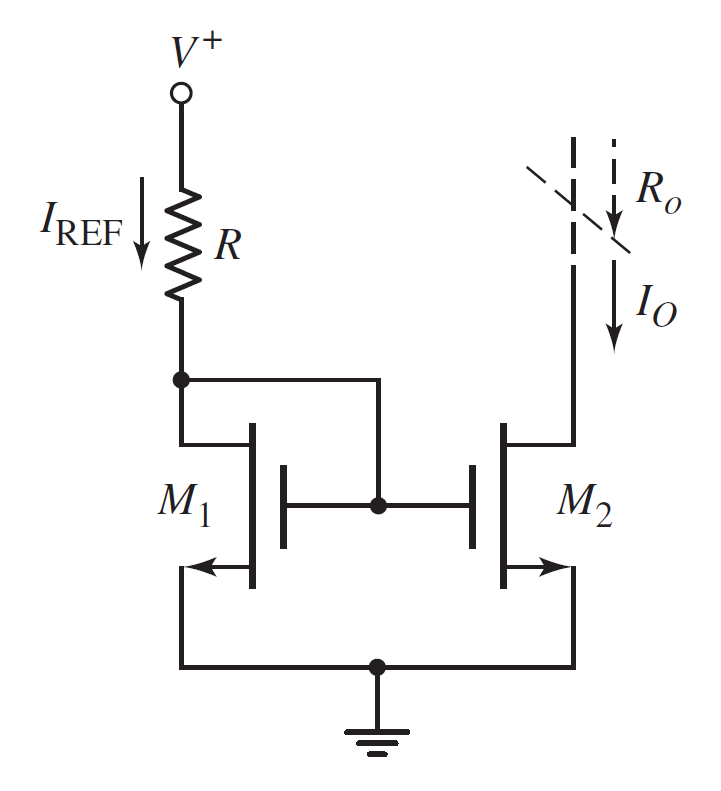
\includegraphics[width=0.4\textwidth]{10.44}
	\caption{Problem 10.44}
\end{figure}
\noindent Solution:

Because of KCL and MOSFET:
$$\frac{V^+-V_{GS}}{R}=K_n(V_{GS}-V_{TN})^2\Rightarrow V_{GS}=1.12\mathrm{V}$$

So $\displaystyle I_{REF}=I_O=\frac{V^+-V_{GS}}{R}=92.05\mathrm{\mu A},V_{DS2(sat)}=V_{GS}-V_{TN}=0.62$V
  
10.54 The transistor circuit shown in Figure P10.54 is biased at $V^+=+5$V and $V^{-}=-5$ V.The transistor parameters are $V_{TP}=-1.2 V, k_p^{\prime}=80\mu A/N^2,\lambda=0,(W/L)_1=(W/L)_2=25,\mathrm{~and~}(W/L)_3=(W/L)_4=4.$ 
Determine $I_\mathrm{REF},I_O$, and $V_{SD2}$(sat).
\begin{figure}[H]
	\centering
	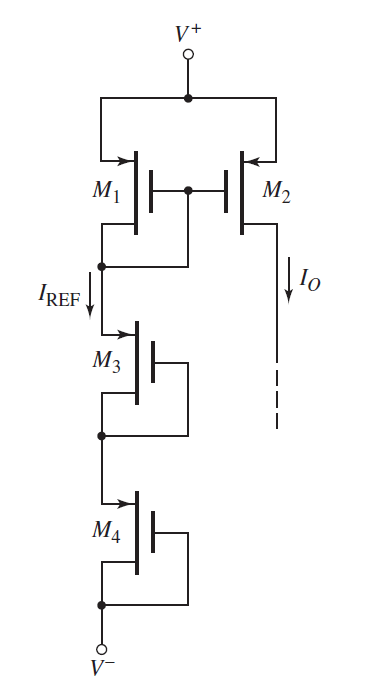
\includegraphics[width=0.4\textwidth]{10.54}
	\caption{Problem 10.54}
\end{figure}
\noindent Solution:

$$\left\{
\begin{aligned}
	&I_{REF}=K_{p1}(V_{SG1}+V_{TP})^2=K_{p3}(V_{SG3}+V_{TP})^2=K_{p4}(V_{SG4}+V_{TP})^2\\
	&V_{SG1}+V_{SG3}+V_{SG4}=V^+-V^-
\end{aligned}\right.
$$
$$
	\Rightarrow V_{SG1}=2.45\mathrm{V},I_{REF}=I_O=1.14\mathrm{mA}
$$

So $V_{SD2(sat)}=V_{SD2}+V_{TP}=1.25$V

10.60 The transistors in the circuit shown in Figure P10.60 have parameters $V_{TN}= 0.4$V$, V_{TP}= - 0.4$V$, k_n^{\prime}= 100\mu$A$/V^2, k_{p}^{\prime}= 60\mu$A$/\mathrm{V} ^2, $and $\lambda_n=\:\lambda_p=0.$ The transistor width-to-length ratios are $(W/L)_1=(W/L)_{2}=20$  $,(W/L)_{3}=5$, and $(W/L)_{4}=10$. Determine  $I_{O}, I_{\mathrm{REF}}, $ and $V_{DS2}( $sat$) .$ What are the values of$V_{GS1}, V_{GS3}$, and $V_{SG4}?$
\begin{figure}[H]
	\centering
	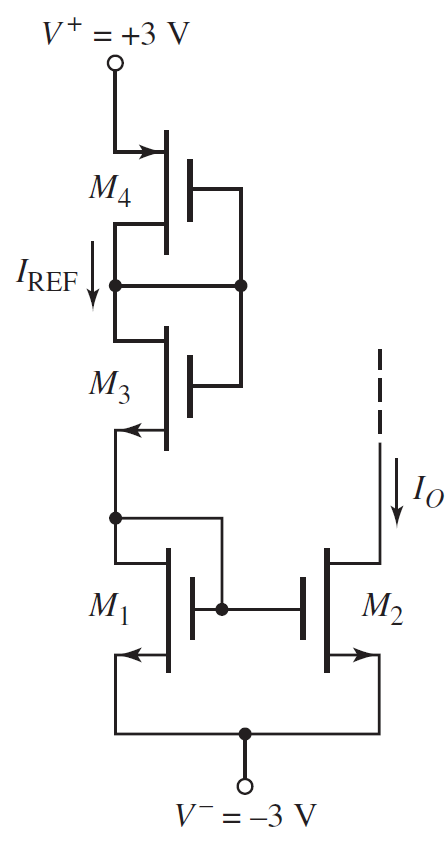
\includegraphics[width=0.4\textwidth]{10.60}
	\caption{Problem 10.60}
\end{figure}
\noindent Solution:

$$\left\{\begin{aligned}
	&I_{REF}=K_{p4}(V_{SG4}+V_{TP})^2=K_{n3}(V_{GS3}-V_{TN})^2=K_{n1}(V_{GS1}-V_{TN})^2=I_O\\
	&V_{SG4}+V_{GS3}+V_{GS1}=V^+-V^-
\end{aligned}\right.
$$
$$	
	\Rightarrow V_{GS1}=1.395\mathrm{V} ,V_{GS3} =2.389\mathrm{V},V_{SG4}=2.216\mathrm{V}
$$
So:
$$
	I_O=I_{REF}=K_{n3}(V_{GS3}-V_{TN})^2=0.99\mathrm{mA}, V_{GS2(sat)}=V_{GS1}-V_{TN}=0.995\mathrm{V}
$$

10.84 In the circuit in Figure P10.84, the active load circuit is replaced by Wilson current source. Assume that $\beta=80$ for all transistors, and that $V_{AN}=120$V, $V_{AP}=80$V and $I_{REF}= 0.2$mA. Determine the open-circuit small-signal voltage gain.
\begin{figure}[H]
	\centering
	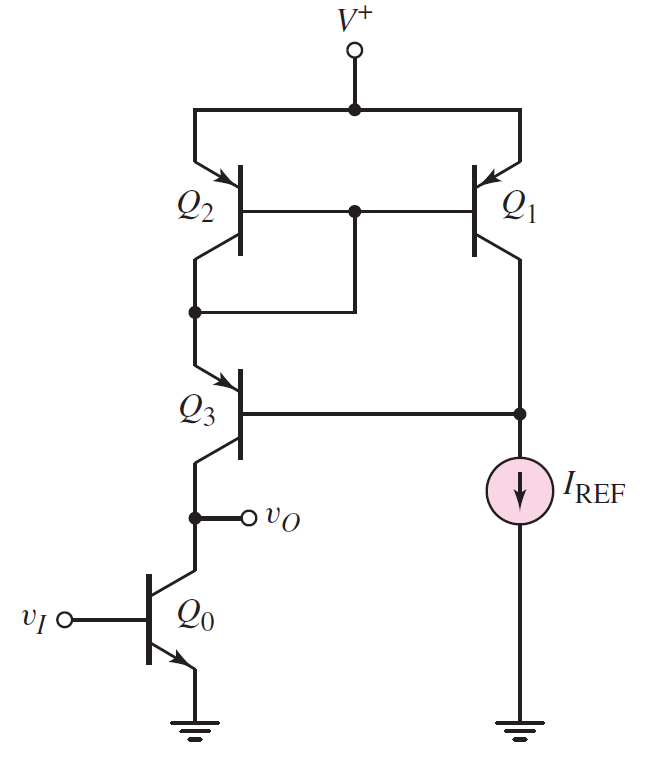
\includegraphics[width=0.4\textwidth]{10.84}
	\caption{Problem 10.84}
\end{figure}
\noindent Solution:
	
Output resistance of Wilson source:
$$
	R_{0}\cong  \frac{\beta{r}_{03}}2  \\
$$

Solve out $g_m$ and $r_{03}$
$$
	r_{03}={\frac{V_{AP}}{I_{_{REF}}}}={\frac{80}{0.2}}=400\mathrm{k}\Omega   \\
	g_{m} =\frac{I_{REF}}{V_{T}}=\frac{0.2}{0.026}=7.692\mathrm{mA/V}  \\
$$

Solve out $A_v$:
$$
	A_{v} =-g_{m}\left(r_{0}\left|\left| \frac{\beta{r}_{03}}2\right.\right.\right)\Rightarrow{A_{v}=-4448} 
$$

\end{document}